\documentclass[12pt,oneside,a4paper]{article}
\usepackage{blindtext}
\usepackage{setspace}
\usepackage[left=1.5in, right=1in, top=1in, bottom=1in]{geometry}
\usepackage{graphicx} %TO include graphics in document
\usepackage{amssymb}
\usepackage{algorithm}% http://ctan.org/pkg/algorithms
\usepackage{algpseudocode}% http://ctan.org/pkg/algorithmicx
\usepackage{url} %for including urls in References
\usepackage{cite}
\usepackage{pdfpages} % To include title page pdf

\begin{document}
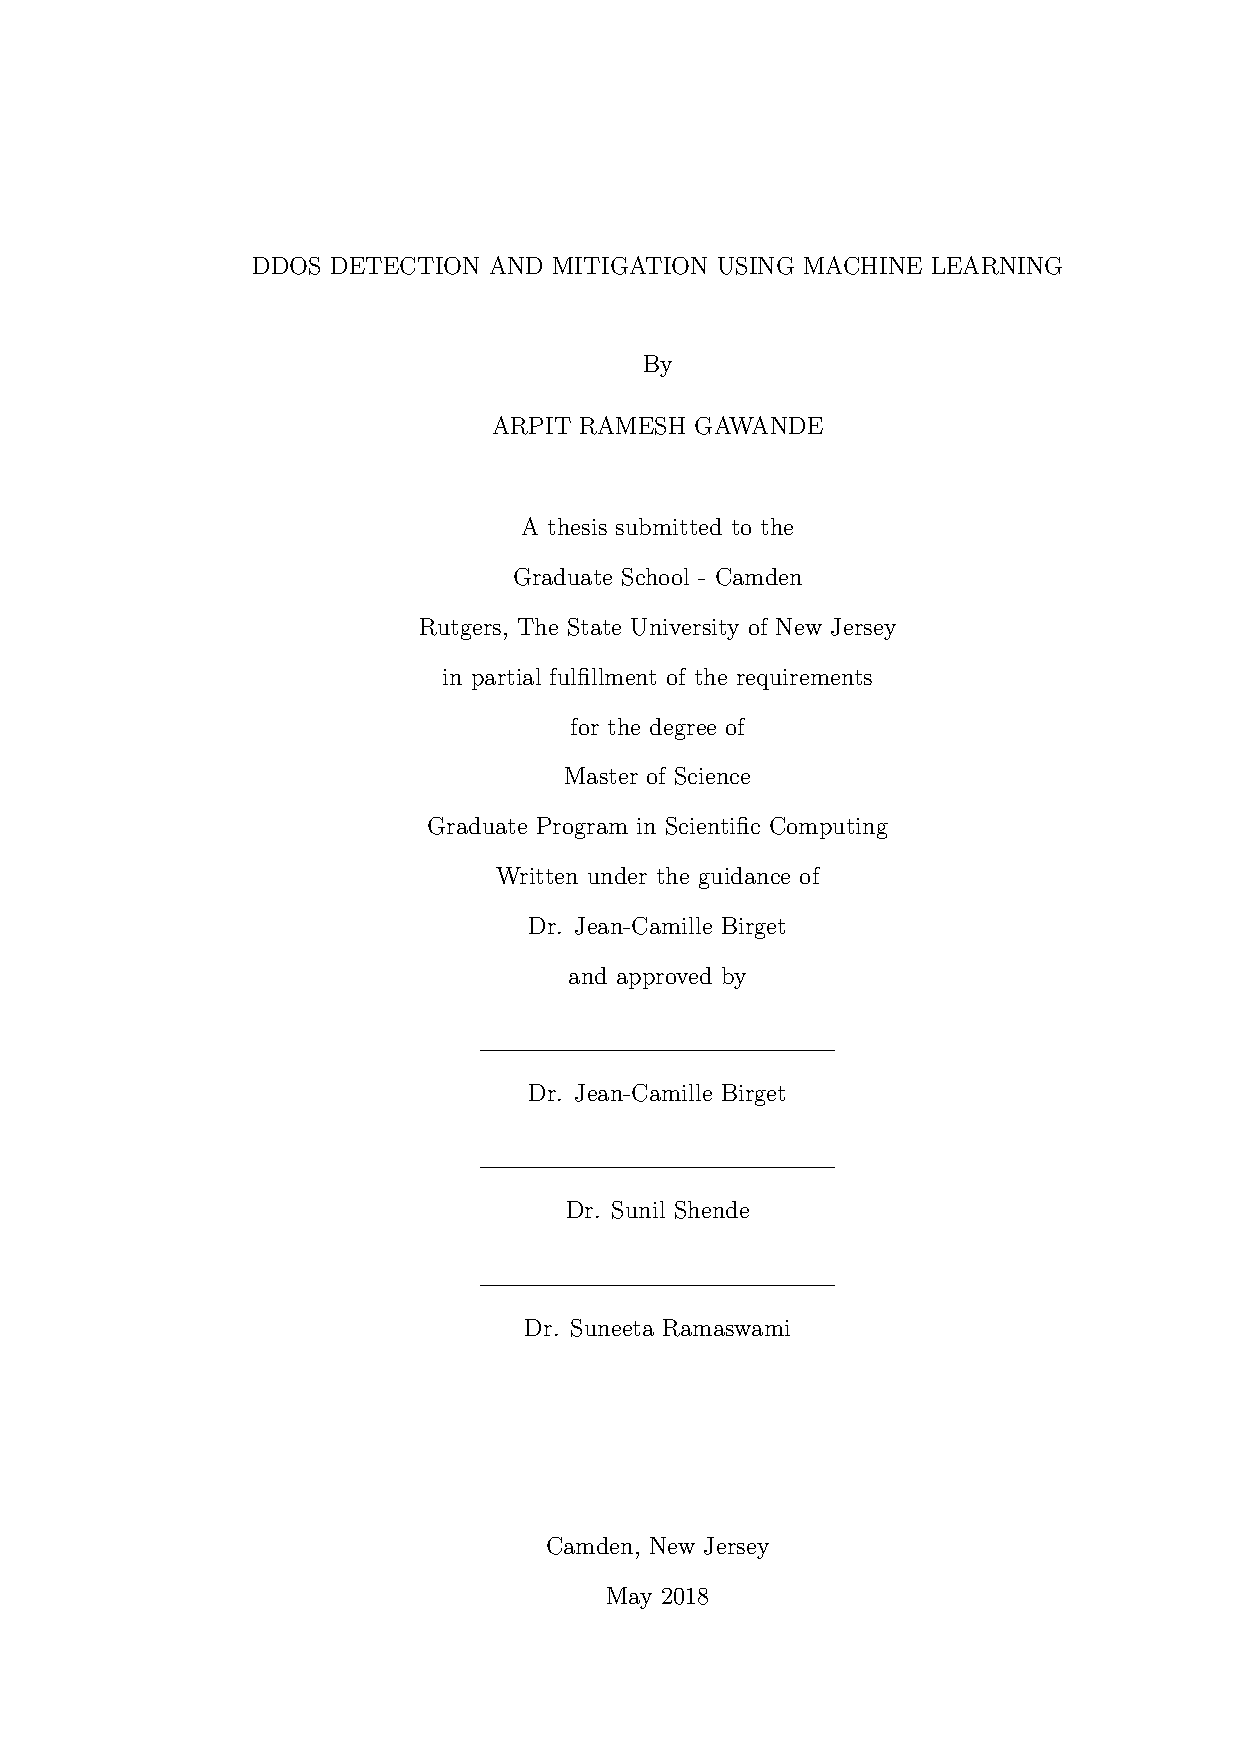
\includepdf{title}
\doublespacing
\renewcommand{\thepage}{\roman{page}}% Roman numerals for page counter
\setcounter{page}{2}% Start page number with 2
\tableofcontents
\newpage
%For page numbering at top right of the page
\pagestyle{myheadings}
\renewcommand{\thepage}{\arabic{page}}% Arabic numerals for page counter

\begin{abstract}
Distributed Denial of Service (DDoS) attacks are very common these days\cite{ddos-attack-news}. It is evident that the current industry solutions, such as completely relying on Internet Service Provider(ISP) or setting up DDoS defense infrastructure, are not sufficient in detecting and mitigating DDoS attacks, hence consistent research is needed. Most of the current industry solutions involve setting up a centralized expensive hardware system which can analyze the data packets \cite{network-data-packet} for probable DDoS attacks. Also each router provider has different protocols to communicate between the DDoS attack detection system and the router/networking devices, limiting the reach of DDoS detection systems. In this paper we have discussed a way to detect DDoS attacks using machine learning tools at the routers, instead of setting a centralized analysis system. Also we have proposed a standard communication architecture which can be used across all the networking devices for mitigating DDoS attacks.
\end{abstract}

\section{Existing Systems}

\subsection{What is DDoS attack}
Distributed Denial of Service (DDoS) attack is a way to jam a host network or its resources with a large number of data packets\footnote{Messages that are sent on the Internet are broken into shorter messages for transmission. These short messages are called packets. Term coined by Donald Watts Davies.} or connections, so that the host becomes disabled. There are different types of DDoS attacks such as :
1. Volume based, e.g. SYN Flood Attacks, in which the victim is flooded with a hight volume of packets or connections.
2. Application based, in which an application such as DNS, VOIP or HTTP are attacked.
3. Low rate DDoS attacks, in which the attacker exploits a vulnerability in the application design, e.g. Slowloris.
\cite{DDoS-attacks}

\subsection{Challenges in dealing with DDoS attacks}
The real challenge in detecting and defending against DDoS attack is because of its dynamic nature. The source\footnote{It is a system/device on the Internet that has an IP address and which is involved in DDoS attack} is not a single node or a system on the Internet but there can be many systems participating in DDoS attack, and often these systems are distributed over different regions of the Internet. Also the source of the packet is often spoofed\footnote{spoofing is the way to change the source IP address of the message. This is a known issue in the protocol itself not in the implementation}\cite{ip-spoofing}, which makes harder to know the actual IP address of the system from where attack is originated because original attack source is changed in spoofed data packet. In addition to that, many times the source system itself is not aware that it is compromised and it is being used as a bot\cite{bot} by an attacker to launch DDoS attack.

As the source address can't be a reliable way to know the attack source (because of spoofing), detecting and mitigating attack at the destination\footnote{System under DDoS attack} is not very useful. Destination may know that the attack is happening but to stop it happening it will have to block all the incoming traffic including the legitimate traffic. To avoid this, many network device producing companies such as Cisco, Netgear have come up with some solutions. Many of the solutions provided by those giants, or the research that is done in this field has been focusing on collecting network traffic flow information\cite{network-traffic-flow} at routers(gateways). A flow consist of a number of Internet packets captured during a fixed time interval. Router send that flow information to the central system for the analysis. Central system is a hardware and software infrastructure which is capable of processing and analyzing large flow information.\par

Some of the major protocols which are widely used for flow collection and analysis are, Internet Protocol Flow Information Export (IPFIX) protocol created by the Internet Engineering Task Force (IETF), Ciscos NetFlow\cite{cisco-netflow} and Sflow(Sampled flow)\cite{sflow}. These protocols have defined standard way to export the flow information from router and similar devices. All these flow monitoring protocols gather information and send the consolidated flow information to the centralized server where user can login and perform functions; such as Security Monitoring, Bandwidth monitoring, Resource Management, Traffic Analysis, Performance Management etc. On such systems, there are some modules which are specifically used for anomaly/DDoS detection.\par

E.g. Cisco netflow has flow exporter, collector and analysis modules. Flow exporter modules are installed on routers. The routers which are having flow exporter modules, send flow information to the collector module installed on the server. Along with the collector module, server also has analysis module which can be used to detect different patterns in the flow.\par

These technologies scales well and can be sufficient to indicate trends in network traffic but they have limitations. 1) They are not cross platform, e.g. router with Sflow protocol can't work with Cisco routers. 2) They involve setting up expensive hardware which acts as collector server. 3) Source address is used for flow analysis which is not reliable due to IP spoofing in the case of of DDoS attack.\par

Now we know that the router based flow analysis can be useful for anomaly detection but it has limitations. We don't want to set up expensive hardware, we want to have a protocol or a system which is compatible with other routers. Also we don't want source IP address for detection analysis. So if we can come up with a way by which we can detect anomaly in the traffic at the intermediate devices on the Internet such as gateway devices(routers) and create a communication protocol between such gateway devices and the destination server or network, then better decisions on regulating the packet flow can be taken.

\section{DDoS Detection and Mitigation}

DDoS attacks can be detected by checking if there is any anomalous behavior in the network traffic, such as, a sudden increase in the number of packets going to a destination. This can be done at the server by observing all the incoming traffic or it can be done by observing all the out going/incoming traffic at the ISP's or at every router. Attack can be mitigated if the anomalous packets are blocked from reaching their destination.

\section{Network Functioning}

A switch creates a network and router connects those networks. A router links computers to the Internet through other routers. Routers are the backbone of the network who helps to forward packet from one point to other point on the Internet. Every packet traveling on the Internet has to go through a router\cite{router-switch}. Router knows where the packet is destine, hence it could serve as first point of knowledge about the change in the packet flow information for a destine network. Each router has interfaces to which hosts or other network are connected. So router is aware to whom it is connected. Router uses protocol to communicate between other networking devices and by that it gathers knowledge about other networks or routers on the Internet. ICMP\cite{icmp} is one of the most frequently use protocol by routers for communication.\par

\begin{figure}[H]
\centering
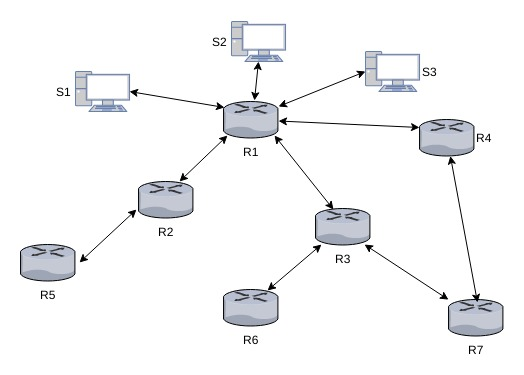
\includegraphics[width=0.70\textwidth]{routers.jpg}
\caption{Network Example} \label{fig:routers}
\end{figure}

Let's illustrate this using an example. In the above figure we can see that host S1, S2, S3 are connected to a router R1. Router R1 is connected to the Internet through router R2, R3 and R4, thus every packet reaching to the system S2 is coming from either of these three routers. All three routers are located in different geographical region. Most of the websites are regional, either county, state or national (If we leave out few global websites) and hence they are mostly accessed from those region it is meant for. E.g. Rutgers University website is accessed mostly from the eastern region of United States and that too mostly from the New Jersey State or the Philadelphia region.\par
Using traceroute we can see how many hops\footnote{hops are intermediate routers in the communication channel} away the destination is. Following is one of the captured traceroute for Rutgers University website.\par
%\vspace{5mm} % vertical space
\begin{figure}[H]
\centering
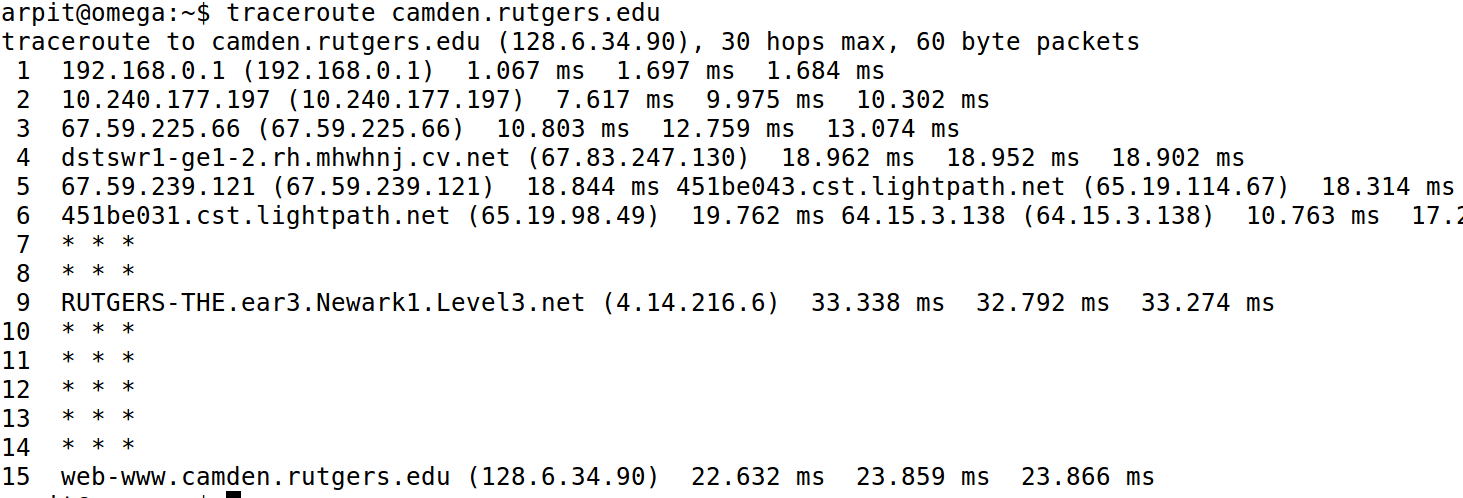
\includegraphics[width=0.90\textwidth]{TraceRoute.png}
\caption{Trace Route: All the routers in the path to destination} \label{fig:traceroute}
\end{figure}

We can see that the packet traverse through the 15 routers to reach to camden.rutgers.edu server. This trace route is taken from a location in the New Jersey State.\par

\section{Our Approach}

\subsection{The router as a point of analysis}
From Figure \ref{fig:routers} and \ref{fig:traceroute} we know that routers are located at different geographical locations and also there are specific regions from which a given website or web server is accessed (except few). There are services called as GeoIP services. They can detect the geographical location of the system from which the IP packet has originated, but that is just an approximate, based on the source IP and not always correct. In case of DDoS attack this information is unreliable, because the packet source address is often spoofed, it is difficult to know the actual geographical location from which the packet has come, but router through which that packet has traveled can provide its own geographical information. Such information can be useful to understand the path through which a packet has traveled and thus we can know the region from which the packet was originated.\par

In the normal scenario there is a consistency in which website is accessed from different geographical regions, and this consistency can be found by measuring the number of requests or packets traveled from a router to a destination server. This behavior of accessing different websites from a router can be learned over the time. Thus finding this behavior in a flow\footnote{In this paper we will consider flow only in the sense of destination addresses} at the router can form the basis of analysis in this paper. If there is a deviation from the learned behavior of accessing a particular destination, then that change in behavior as well as router geographical region information can be communicated to the destination network. The destination network on receiving that information, can decide, whether it wants the reporting router to discard or forward the traffic for it. This is a selective process in which traffic from only specific router is blocked while traffic from other routers remain unaffected\par

With the advance of electronics and the Internet of Things, processing and storage capacity of the electronic devices has increased. Routers are also not left behind, but storage capacity of routers is always very less compared to server which collect flow data for network traffic analysis. If we use learning techniques that don't need much storage then we don't have to store large chunk of packets on the router. Instead of storing data packets for longer time for analysis, we can learn from a small number of packets and then discard packets once learning is done, leaving behind only the learned information on the router. This is necessary because the number of entries on the Internet routing table has steadily grown. Now that the table has passed 500,000 routes\cite{routing-tablesize}, so storing each and every flow information for these routes could be difficult.\par

\subsection{Internet packet flow capturing at the router}

\begin{figure}[H]
\centering
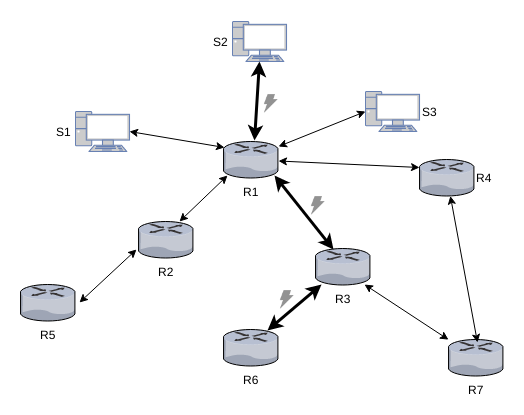
\includegraphics[width=0.70\textwidth]{attack_path.png}
\caption{DDoS Attack path} \label{fig:attackpath}
\end{figure}


In the above figure an attack is initiated from the region where router R6 is located and from router R6 data packets travel to the victim\footnote{Victim is a computer system which is under DDoS attack} system S2. Attack packets traveled through router R3 and R1 to reach system S2. If we can detect an attack at router R6, then router R6 can discard all the packets heading towards system S2. In this process, only traffic from router R6 is affected but traffic from all other routers remain unaffected.

To achieve this, we will gather the flow information during a time window (e.g 300 sec) whose size will be fixed at the beginning. Thus a flow will contain all the packets that traveled from a router to different destinations during a time span of 300 seconds. We can also combine such flows to form a new flow with bigger time windows. E.g. if we combine two flow of 300 seconds then we will have flow of 600 seconds. This flow information can be capture during a particular period or throughout the day. Once we have flow information we can apply learning techniques on each flow iteratively to gain deeper knowledge about normal behavior of the flow, e.g. on average, how many packets of different protocols are destined for a given destination from a given router/region during a particular time of the day.

\begin{figure}[H]
\centering
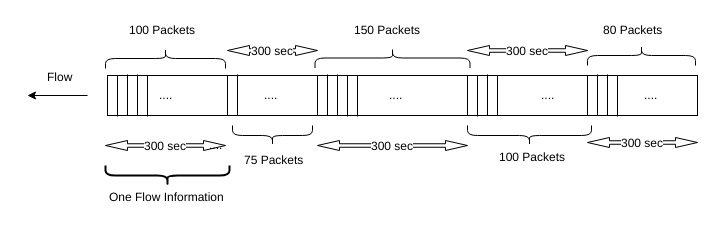
\includegraphics[width=0.90\textwidth]{Data_Flow_Capture.png}
\caption{A 300 second time segment corresponds to a flow of information. The number of packets can vary in a flow.} \label{fig:flow}
\end{figure}

\subsection{Analysis techniques to be implemented}
In the proposed system, each router will itself act as an analyzer. Each packet will be analyzed and a flow statistic will be created based on the destination IP address. Flow statistic will be used to create feature vectors and those feature vectors will be used for clustering destination IP address. Clustering is a process of examining the collection of “points,” and grouping the points into “clusters” according to some distance measure. The goal is to minimize the distance of every point in the cluster to other points in the same clusters.\cite{machine-learning}.

Once the clustering is learned (i.e. we know which destination IP address is tend to be in which cluster), the learned information will be used as a benchmark for all future flows. The routers will constantly keep clustering destination IP addresses and if there is deviation for the normal traffic at a router for any destination then that will affect the clustering and it will cause the destination IP address to be placed in different cluster. This change in the cluster for a given destination IP address can be marked as a change in the behavior of the traffic for that destination. Along with the cluster we will also use the Novelty Detection algorithm to achieve more accurate result. This change in traffic behavior will be reported to destination network, which then decides on regulating the traffic coming to itself from the router which has sent the information.

\section{Implementation} \label{sec:Implementation}

As discussed previously, there are different types of DDoS attacks, such as volume-based, application-based and also low-rate DDoS attacks. Among these different types of DDoS attacks, the volume-based attacks are most common. In the volume-based attack, a victim is flooded with a high volume of Internet packets (TCP, UDP, HTTP or ICMP), which make it unable to serve the requests.

For the demonstration of the suggested approach we are simulating a volumed-based bot attack. In the real world, the volume-based attacks are orchestrated using bots. Bots use compromised computer systems, controlled by an attacker for launching an attack. They are not bounded by geographical boundaries, so they can be anywhere in the Internet. Botnet (i.e. network of bots) are employed by an attacker to launch a DDoS attack. As we know that the Internet is connection of different computer system that communicate with each other, through different channels such as cables, satellite or radio device and these communication channels run throughout the glob; connecting different computer systems at different locations. For our simulation, instead of any bot program, we are using Low Orbit Ion Canon(LOIC) tool which is a free DDoS attack launching tool. This tool is even used by attackers in the real world to launch DDoS attacks.

We used Wireshark, an open source tool, for capturing Internet packets. Wireshark can capture all digital information received or sent through different devices such as Ethernet or wifi devices, which connect computers to the Internet. It also helps identify different protocol packets (e.g. TCP, UDP) within the wrapper packet created at Data Link Layer packet.\par

\begin{figure}[H]
\centering
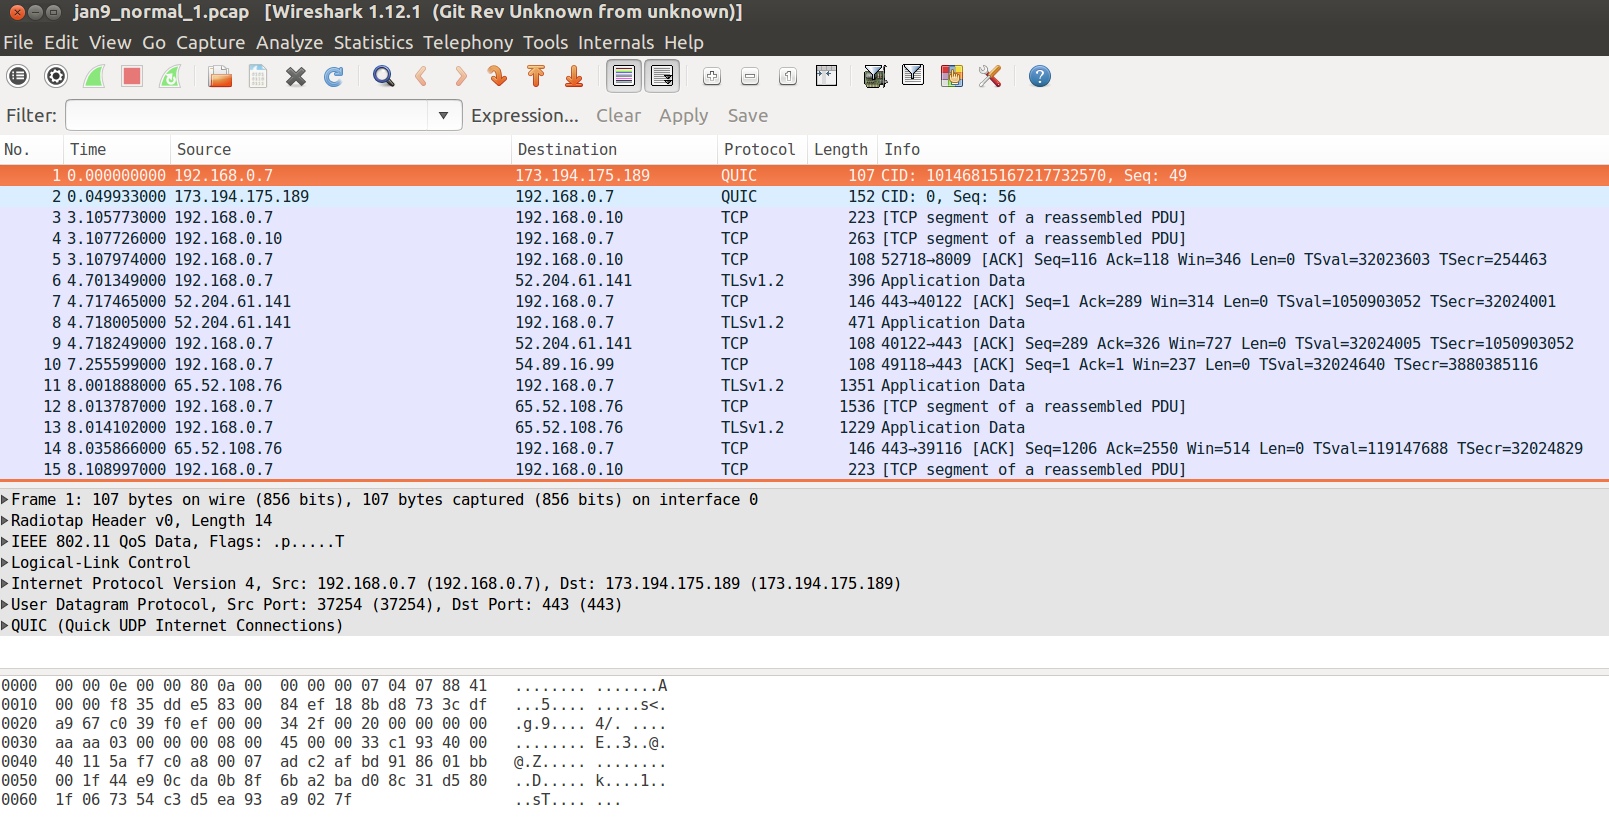
\includegraphics[width=0.90\textwidth]{Wireshark_Tools.png}
\caption{Wireshark Tool: snippet of captured packets} \label{fig:wireshark}
\end{figure}

To gather data for the demonstration, we have created a small network which has one router and couple of host machine. Each machine can be a victim of a DDoS attack. We have installed Wireshark tool on one of the machine in the this network. For capturing traffic in the network we are using the Promiscuous mode of Wireshark. In Promiscuous mode, a network interface can record not only the traffic that is intended to itself but all of the traffic on the network, so we can see all in/out traffic in our setup network. This setup is similar to any router on the Internet which is connected with different routers and hosts.

\begin{figure}[H]
\centering
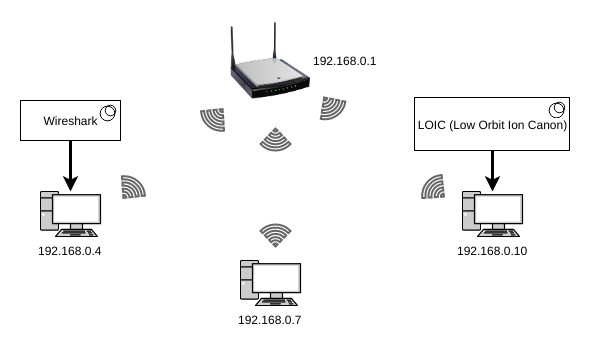
\includegraphics[width=0.90\textwidth]{demo_network.png}
\caption{Network for simulating DDoS detection} \label{fig:demonetwork}
\end{figure}

To collect packets traveling in our network, we start the Wireshark tool. We let it run for a while and then we orchestrate a DDoS attack on one of the host (e.g. 192.168.0.7 in Figure \ref{fig:demonetwork}) in the network. This attack is engineered using the Low Orbit Ion Canon(LOIC) tool that is installed on one of the host (e.g. 192.168.0.10 in Figure \ref{fig:demonetwork}) in our network. This tool allow us to launch TCP and UDP flood attack on any destination. In this paper we are analyzing the flow based TCP and UDP attack, which is one of the most common type of DDoS attacks.

In the LOIC tool we need to give the IP address and the port number of the destination where we want to orchestrate attack while rest of the work is done by it. This tool floods destination with packets and if we choose TCP then it will try to create multiple connections and send packets over them. We start flood attack on one of the system(e.g. 192.168.0.7) in demo network and let it continue for few minuets. We launched such attacks few times in between the packet capturing session.

All the traffic, including the normal and the attack traffic, will get captured using Wireshark. Packets are captured for about five hours in the given network. Once the packets are captured they are saved as pcapng file, which is a Wireshark file format for captured packets. Captured packets during the normal operation and during the attacks are saved separately. The normal packet flow information is used for training and testing the learning algorithms (we will explain it in later sections) while attack packets flow information is used for detecting the attack. Wireshark captures every detail of the packets but we don't need all of the information, we are interested only in the IP layer information of the packet. Most of the routers analyze IP layer of the packet for routing, having said that, there is no reason that other layers of the packet can not be analyzed, but for our demonstration purpose we are analyzing only IP packets.\par

A data extraction program is written in Python language to extract IP layer information from the captured packets. This program extracts address, port and time information from each of the captured IP packets\footnote{packets containing IP information}.

\begin{table}[H]
\centering
  \begin{tabular}{| l | c | l | c |}
    \hline
    Destination IP Address      & Protocol  & Time stamp(Sec.)  & Sample Number \\
    \hline
    52.6.129.72         & 6         & 1512094785.928596000  & 1 \\ \hline
    192.168.0.4         & 6         & 1512094785.946987000  & 1 \\ \hline
    192.168.0.4         & 17        & 1512094786.148488000  & 1 \\ \hline
  \end{tabular}
\caption{Sample file snippet (row represents an IP packet)} \label{table:sample-file-snippet}
\end{table}

Our data extraction program also divides the captured data into 300 seconds capture window, thus creating a sample data which is a collection of IP packets captured over the time of 300 seconds. It then writes each sample in the separate file for further processing. This sampling of the packets is the continuous process. We then run another program which extracts the flow information from those sample files. One `flow' contains the number of different packets capture for a given destination. We will store this flow information as sample flow. Then we will train learning algorithms using those sample flows. Once learning is done, those sample files will be discarded and new samples will be created for further training. This training process has to be continuous process in order to correctly reflect the current status of the flow at given router. Whatever the new information learned, is augmented with the previous learning to have the correct understanding of the flow. This learning can be done for the time during a day or during a week of a year. E.g. We can have separate learning information for flow from morning 9 am to 12 pm and also can have information for evening 6 pm to 12 pm.

Flow based model is built, as it is more reliable and fast. Packet analyzing is often difficult due to the size and encryption. Also destination port number is not a reliable information in detecting attacks because of the fact that attacker uses different ports during an attack.

Creating a training set for the learning algorithms is an intermediate step in which IP packet count for each destination for a given protocol(e.g TCP, UDP) is calculated. The training set gives us the flow information for each destination (i.e. how many packets of a particular protocol are recorded for a given destination IP address during a time window e.g. 300 seconds).

\begin{table}[H]
\centering
  \begin{tabular}{| l | c | c | c |}
    \hline
    & \multicolumn{3}{ |c| }{IP Packet count} \\ \cline{2-4}
    {Destination IP Address}  &ICMP  &TCP &UDP\\
    \hline
    172.217.10.134  & 0     & 8     & 12 \\ \hline
    65.19.96.252    & 5     & 0     & 192 \\ \hline
    68.67.178.134   & 0     & 78    & 0 \\ \hline
  \end{tabular}
\caption{Training Set with three training examples} \label{table:feature}
\end{table}

We are using Python program to create training sets, as given in above table \ref{table:feature}, from the sample files. Each row in a training set is one training example with destination IP address as label. A training example is $\mathbb{R}^3$ vector whose elements are the number of packets observed for a particular protocol for a destination during a fixed time (e.g. 300 second). There are around 150 protocols managed and assigned by the Internet Assigned Numbers Authority (IANA) but most commonly used protocols in the DDoS attack are ICMP, TCP and UDP protocols. For the training and analysis purpose we are using only these three protocols as the desired feature. In the larger system such as routers managed by ISP, other protocols can also be used as features if required.

Each sample file is processed and corresponding train/test set file is created. Train and test sets files are stored on the file systems, so that those can be used by other programs for training and testing the learning algorithms.

\subsection{Machine Learning}

According to Tom Mitchell (1998), a computer program is said to learn from an experience E with respect to some task T and some performance measure P, if its performance on T, as measured by P, improves with experience.

A learning algorithm builds a hypothesis using a training set as input. Then that hypothesis is used to perform predictions. The most common categorization of machine learning algorithms is Supervised and Unsupervised.

Let $f$ be the function from $\mathbb{R}^d$ to $\mathbb{R}^d$ which we need to guess from an input vectors $x^{1}, x^{2}, ..., x^{n}$ also called as `input variables' or `feature vectors'. Let $\Xi$ be the set of such input vectors. Let be the $n$ number of input vectors in a training set $\Xi$. Let $H$ be the set of some functions from $\mathbb{R}^d$ to $\mathbb{R}^d$. Let $h \in H$ be the hypothesis about function $f \in H$. We select $h$ based on a training set $X \in \Xi$, of $m$ input vectors. In Supervised leaning we know the values of $f$ for $m$ samples in the training set $X$. We assume that if we can find a hypothesis $h$ that closely agrees with $f$ for the members of $X$, then this hypothesis will be a good guess for $f$ when $X$ is large. In Unsupervised learning, we simply have a training set of vectors without function values for them. The problem in this case, typically, is to partition the training set into subsets, $X_1,.. ,X_{N}$, in some appropriate way.\cite{machine-learning}

A supervised algorithm such as One Class Support Vector Machine (SVM)\cite{svm} is efficient at identifying the anomalies in the data but this algorithm is process and memory intensive, so training the algorithm for each and every IP address is very costly in terms of resources. Because of the resource constraints of the router, our approach is to first cluster the IP addresses based on the features using Unsupervised learning algorithms such as k-means and then apply One Class SVM on the clusters to decide on the boundaries of those clusters. The k-means algorithm is fast and consumes less resource compared to One Class SVM, that makes it good choice to be used on the devices such as routers which have less processing power and less memory.

\subsubsection{Feature Scaling}

Before feeding training data, which was acquired in an earlier stage, to a learning algorithm, we have to do feature scaling, also called Standardizing. Feature scaling is done by subtracting the mean and scaling the feature to a unit variance value. It is necessary because  different features which are at different scales could cause one feature dominating the others in the algorithm output result. e.g. consider two vectors (1, 2, 3000) (1, 3, 2000). If we calculate the Euclidean distance between these two vectors using the formula $\sqrt{\sum_{i=1}^n (p_i - q_i)^2}$, then the distance will be $\sqrt{(1-1)^2 + (2-3)^2 + (3000-2000)^2}$ . Form this, it is evident that the larger term is dominating the result.

First we will convert training examples into a vectors. Each vector is one training example and each coordinate in the vector is the feature. To standardize the input vector, the mean and the standard deviation are calculated for the set of input vectors. Then a new vector is created by subtracting the mean from each feature vector and dividing that feature vector by its standard deviation. The new vector created after this step is standardized vector. A set of such standardized vectors is used as input to the learning algorithms.

\hspace{2cm} Standardization formula: $x' = \frac{x - \bar{x}}{\sigma}$

Where $x$ is a feature vector, ${\bar{x}}$ is the mean and $\sigma$  is its standard deviation.

\subsubsection{Clustering} \label{subsec:Clustering}

k-means\cite{k-means-clustering} clustering is one of the most efficient algorithms for creating clusters. This algorithm takes any $k$ randomly chosen points as centroids (also called, cluster centers) $\mu_{1}, \mu_{2}, ..., \mu_{k}$ as input from the training set $X = \{x^{1}, x^{2}, ..., x^{m}\}$, $x^{i} \in \mathbb{R}^d$, $i= {1,2, ..m}$.

The following is Lloyd's algorithm which is most popular heuristic algorithm for k-me—ans clustering. The clustering that we will be doing is of destination IP addresses, such that each cluster will have some number of destination IP addresses.

\begin{algorithm}[H]
\caption{k-means}\label{k-means}
\begin{algorithmic}[1]
  \Repeat
  \State{Calculate the distance for each element (or data point) of the training set to all the centroids}
  \State{For each element, assign the element to the centroid which is nearest}
  \State{Recalculate the new centroid for all the element in one cluster by taking the mean. If ${x^j_1, x^{j_2}, ..., x^{j_n}}$ are the elements of the cluster $j$. Then for cluster $j$, the new centroid will be $\mu_{j} = \frac{1}{n} [x^{j_1} + x^{j_2} + ... + x^{j_n}]$ where $n$ is number of point assigned to cluster $j$. Do this for all the clusters}
  \Until{No data point is reassigned to a different centroid}
\end{algorithmic}
\end{algorithm}

For this paper we will be using the k-means++ algorithm\cite{k-means++} which is an improvement of k-means, where an arbitrarily initialization step is replaced by simple, randomized seeding technique. If $D(x)$ is the shortest distance from a data point $x \in X$ to the closest centroid we have already chosen, then the following is the k-means++ algorithm.

\begin{algorithm}[H]
\caption{k-means++}\label{k-means++}
\begin{algorithmic}[1]
  \State{Take one centroid $\mu_1$, chosen uniformly at random from $X$}
  \State{Take a new centroid $\mu_j \neq \mu_1$, by choosing $\mu_j \in X$ with probability $\frac{D(\mu_j)^{2}}{\sum_{x \in X} D(x)^{2}}$}
  \State{Repeat Step 2. until we have taken $k$ centers altogether}
  \State{Proceed with the Lloyd's k-means algorithm skipping random the initialization stage}
\end{algorithmic}
\end{algorithm}

For our DDoS attack detection program, we will be using the Scikit-learn libraries. Scikit-learn is the most popular and rich open-source machine learning software library for the Python programming language and it has implementation for both k-means++ and One Class SVM machine learning algorithms, also it has data preprocessing programs such as feature scaling.

We will take a training set (in the format given in figure \ref{table:feature}) and we will cluster training examples from that training set to using the k-means++ clustering algorithm from Scikit-learn library.

\begin{figure}[H]
\centering
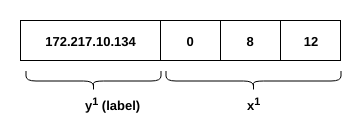
\includegraphics[width=0.70\textwidth]{training_example.png}
\caption{One training example} \label{fig:training_example}
\end{figure}

Before doing the clustering, we have to first determine the number of clusters and centroids.\footnote{Centroid is the vectors which is arithmetic mean of all the point in the cluster} Deciding on the number of clusters is important, because randomly choosing the number of clusters will not have correct clustering. So, we will use the Elbow method to find the optimal number of clusters in our training set. The Elbow method checks the portion of the variance explained by function of the number of clusters. Following are the Eblow Diagrams for four samples.

\begin{figure}[H]
\centering
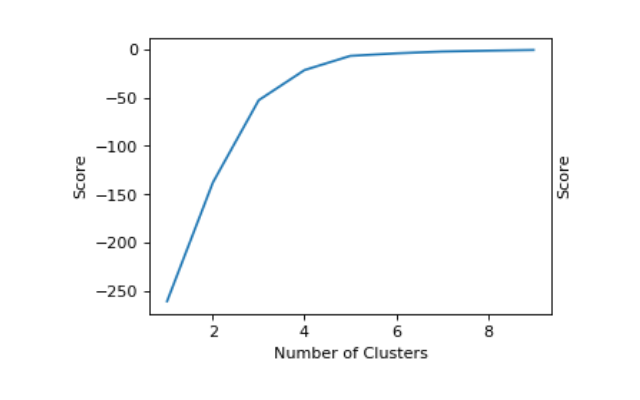
\includegraphics[width=0.90\textwidth]{elbow-method.png}
\caption{Elbow Method for cluster count detection} \label{fig:elbow-method}
\end{figure}

Using the elbow method, the variance for each cluster number is calculated and the cluster number which produces less variance for the next cluster number is selected as best choice for the give training set.

To have correct clustering we first run the k-means++ algorithm to determine the central vectors called centroids. Clusters are represented by these centroids. As we have multiple training sets (also called `samples'), we have cluster centroids for each sample. But in the future we will require only one set of centroid which would be the more accurate clustering for all our training sets. To achieve this, we will save all the centroids, and then find the median of those centroids after removing the outliers, and that will give us a good estimate of centroids. This estimated centroids are used for clustering the samples in the future. Following is the example of centroid vector, where a rows represents a cluster and a column represents a feature.

\begin{table}[H]
\centering
  \begin{tabular}{ l | c  c  c }
    Cluster      & ICMP  & TCP  & UDP \\
    \hline
    0         &{-0.16815612}       &{-0.14928111}    &{-0.16948046} \\
    1         &{-0.18181818}       &{5.13527652}     &{5.68956244} \\
  \end{tabular}
\caption{Example of cluster centroids: A row is a cluster and column is a feature} \label{table:centroids-example}
\end{table}

Once we have centroids we can use them to cluster training set again and get the correct clustering based on the centroid.

After clustering is done, it needs to be tested for the accuracy. I.e. how similar the test set clustering is with training set clustering. This can be done by checking, whether an IP address has the same cluster number assigned in both the training and the test sets or it differs. For measuring this similarity, Rand Index(RI)\cite{ri-index} is used. RI is a measure of how many percent does the test clustering matches with the trained model.

\hspace{4cm} $RI={\frac {TP+TN}{TP+FP+FN+TN}}$

where $TP, TN, FP$ and $FN$ are the number of true positives, true negatives, false positives and false negatives respectively.

Because of the training sets contain the flow information for different IP addresses on a router during the window of 300 seconds, there is a very high possibility that the same destination IP address is captured in multiple training set. Our goal is to find the correct cluster for the destination IP address, and to achieve this goal, we have labeled IP address with cluster in which it is found most of the time in all our training sets. E.g. If an IP address is assigned cluster `0' in five training sets and cluster `1' in two training sets, then that IP address would be assigned cluster `0' in the result, that we store for future referencing.

\begin{table}[H]
\centering
  \begin{tabular}{| l | c | c | c | c |}
    \hline
    {Destination IP Address}  &Cluster  &Packet Count \\
    \hline
    74.125.141.106  & 1     & 113  \\ \hline
    72.30.2.182     & 0     & 16   \\ \hline
    64.94.191.14    & 0     & 22   \\ \hline
  \end{tabular}
\caption{Learned information after clustering} \label{table:learned-clustering}
\end{table}

The clustering information tells us the normal behavior of the packets traveling from the router to a given destination. As we have fixed the centroids for the clustering, every time in the future we should expect an IP address to be found in the same cluster mentioned in the clustering information table. But If there is a DDoS attack on a any destination with flooding, then we can expect to see the destination IP address assigned to different cluster.

\subsubsection{Anomaly Detection using One Class Support Vector Machine} \label{subsec:Anomaly_Detection}

\paragraph{Support Vector Machine:}

From the experiments on different data sets, it is found that the destination under attack is labeled with the same cluster number. This happened because there is no other cluster it can be assigned to, so it gets assigned to the cluster whose centroid is nearest.

To avoid such a situation, we will have to create boundaries for the clusters, and if any IP address is outside of the cluster boundaries then that can be considered suspicious. This provision will make sure that the attack on the destination IP address will be detected even if the destination is assigned to the same cluster it was assigned in the past.

To create cluster boundaries we have used One Class SVM classifier. One Class SVM is a supervised machine learning algorithm, which means, the training example will have label. I our case, a cluster number will be treated as label for a training example (see table:labeled-set).

One Class SVM is a type of Support Vector Machine (SVM). SVM is a supervised learning algorithm which tries to classify training examples into two distinct classes. Classification is based on the labels of the training set.
Consider the training set $\{(x^{1},y^{1}), .., (x^{m},y^{m})\}$, where $x^{i} \in \mathbb{R}^d$ is the training example and $y^{i} \in \{-1, +1\}$ is a label (or a class) for $x^{i}$. SVM will separates those classes using a line or a curve.

SVM tries to create a non-linear separation boundary by projecting data points through a non-linear function $\phi$ (kernel function) to higher dimension space. The data points in space $I$ which can't be separated by a line are projected to the feature space $F \in \mathbb{R}^d$ where there can be a hyperplane that separates data points of one class form another. If that separating hyperplane is projected back on the original space $I$ then we get a non-linear curve.\cite{svm}

\begin{figure}[H]
\centering
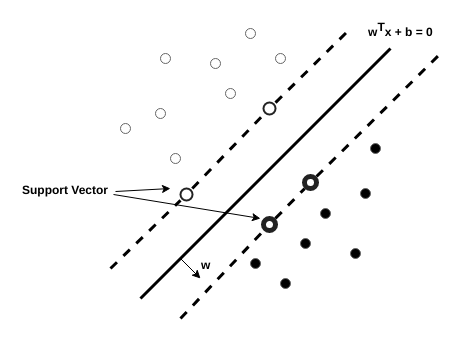
\includegraphics[scale=0.5]{SVM}
\caption{Linear Separation using Support Vector} \label{fig:SVM}
\end{figure}

The hyperplane is represented with the equation $w^{T} x + b = 0$, where $x \in \mathbb{R}^d$, $w \in F$ and $b \in \mathbb{R}$. This hyperplane separates the training example labeled with $-1$ and $1$. The position of the hyperplane is such that the distance from the closest point from each class to the hyperplane is same. To avoid the over-fitting, slack variables $\xi^{i}$ are introduced. Over-fitting happens because the learned hypothesis fits training examples so well that it fails to generalize the new examples. The SVM classification is an optimization problem which is stated as follows.\cite{svm} \cite{svm-ml}

\begin{center}
  ${min}_{w,b,\xi^i} \ \frac{||w||^2}{2} + C \sum_{i=1}^m \xi^i$ \\
  $\mbox{ subject to: }$ \\
  $y^i( w^T \phi(x^i) + b) \geq 1 - \xi^i \mbox{ for all } i = 1, \dots, m$ \\
  where $y^{i} \in \{-1, +1\}$, $x \in \mathbb{R}^d$, $b \in \mathbb{R}$ and $\xi^i \geq 0 \mbox{ for all } i = 1, \dots, m$ \\
\end{center}

 $\phi$ is a kernel function and constant $C > 0$ is the regularization parameter. If $C$ is chosen large, miss-classification of training examples can be avoided. If chosen small, then we may miss-classify few examples, but the margin will be large, so most of the points will be far away from the decision boundary. If this minimization problem is solved using Lagrange multipliers then the classification function is:

\begin{center}
$sign(\sum_{i=1}^m \alpha^i y^i K(x,x^i) \ + \rho)$
\end{center}

$\alpha^i$ is the Lagrange multipliers. $\alpha^i y^i$ called the support vectors. The function $K(x,x^i)=\phi(x)^T \phi(x^i)$ is the kernel and $\rho \in \mathbb{R}$ is the intersection.

\paragraph{One Class Support Vector Machine:}

One Class Support Vector Machine (SVM) is the extension of SVM which detects boundaries of the training set so that every new training example will be classifies as belong to training set or not. It separates all the training set data point from feature space $F$ and maximizes the distance of hyperplane from $F$. This creates a binary function which returns +1 for the training example that fits in the trained set region, otherwise it will return -1.

The minimization function of One Class SVM is slightly different than the SVM. \cite{svm}

\begin{center}
  ${min}_{w,\rho,\xi^i} \ \frac{||w||^2}{2} + \frac{1}{\nu m} \sum_{i=1}^m \xi^i - \rho$ \\
  $\mbox{ subject to: }$ \\
  $(w.\phi(x^i)) \geq \rho - \xi^i \mbox{ for all } i = 1, \dots, m$ \\
  \hspace{2cm} $\xi^i \geq 0 \mbox{ for all } i = 1, \dots, m$ \\
\end{center}

The new parameter $\nu \in (0,1]$ introduced in place of $C$ in previous SVM equation is used to set upper bound on outliers/anomalies and lower bound on the number of training examples.

Because SVM solves a quadratic programming problem (QP), computing and storage requirements of SVM increases rapidly with the number of training vectors. The approach presented in this paper is more efficient because the number of cluster are limited and always be far less than the number of destination IP address. Training one class SVM on clusters will be far less process and memory intensive than training on massive number of IP addresses. E.g. In our simulation training sets we have 4 four clusters, while the unique number of destination IP addresses in all the training sets is 268, which is more than 60 times the count of clusters we have found.

To classify whether a test example can be a part of a cluster, we need to have classifier for each cluster. I.e. If we have four clusters, we need to train four One Class SVM classifiers, one for each cluster.

\section{Detection} \label{sec:Detection}

To detect an attack, we have to capture the packet flow at the router during a time interval with which we have created our trained set (e.g. 300 second window). We have to transform the captured flow into a test set using same programs we have used to create training sets from the sample files. The created test set is then clustered using the kmeans++ algorithm, using the centroids, that were found after clustering the training sets. We then check the cluster assignment for each example in the test set, and if there is any destination IP address\footnote{a destination IP address is a label of a test example} for which the new cluster assignment does not match with the already known cluster for that destination IP address, then that destination IP address is suspected to be under the DDoS attack and so it is added to the suspect list. The suspect list will contain the IP addresses which are probably under DDoS attack, because they are not in the cluster they are supposed to.

In another scenario, If the test cluster label for an IP address matches with the trained cluster label, then the feature vector for that destination IP address is passed to the cluster classifier to check if it is inside the boundary of that cluster. As explained in previous section, we will use One Class SVM classifier to decide the boundaries. E.g. if an IP address is labeled with cluster number 0, then we will use One Class SVM classifier that was trained on cluster 0. If the output of the classifier is -1 then that destination IP address is added to the suspect list. Failing to be in the same cluster boundary, that it was in the past, is a sign of significant change in the behavior of the traffic for a given destination IP address on the router where this analysis is done. For every destination from the compiled suspect list, the total number of packets observed in the test set are also recorded. The packet count will act as a filter, to eliminate any misclassification. If there is a significant difference between the number of captured packets in the training and in the test then that destination IP address will be considered under DDoS attack.

\section{Detection Simulation}

We have created a simulation for detecting DDoS attack using the approach proposed in this paper. As explained in section~\ref{sec:Implementation} on page \pageref{sec:Implementation}, we have a small network of three computers and a router. We captured the normal as well as orchestrated DDoS attack traffic in the network. We processed the capture data, converted it into samples and use those samples to create training sets. We are using training sets created from the normal traffic for labeling IP addresses with cluster numbers, and then training the classifiers.

We have first used the elbow method explained in section \ref{subsec:Clustering} on page \pageref{subsec:Clustering} to detect the optimal cluster count. Using that method, we were able to detect 4 clusters in our training sets.

\begin{figure}[H]
\centering
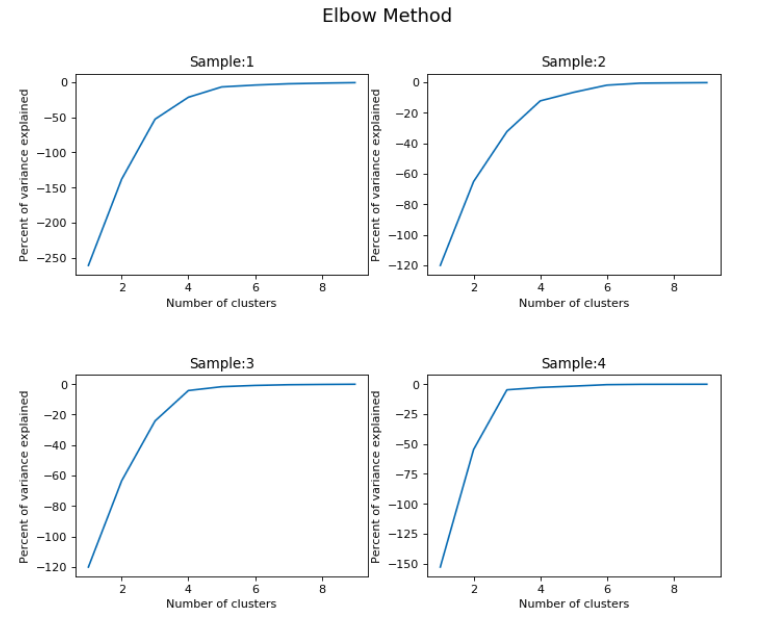
\includegraphics[width=0.90\textwidth]{elbow-method-applied.png}
\caption{Elbow method to find number of clusters}
\label{fig:elbow-method-applied}
\end{figure}

We then applied kmeans++ clustering, as explained in section \ref{subsec:Clustering} on page \pageref{subsec:Clustering}, to find the correct centroids for our training examples. We found following centroids for our training sets.

\begin{table}[H]
\centering
  \begin{tabular}{ l | c  c  c }
    Cluster      & ICMP  & TCP  & UDP \\
    \hline
    0         &{-0.16815612}       &{-0.14928111}    &{-0.16948046} \\
    1         &{-0.18181818}       &{5.13527652}     &{5.68956244} \\
    2         &{5.08663322}        &{-0.27110845}    &{-0.099885} \\
    3         &{-0.18670401}       &{-0.18804342}    &{-0.018538} \\
  \end{tabular}
\caption{Cluster centroids for our training examples} \label{table:centroids}
\end{table}

We then used these centroids to cluster our training sets. To draw the clusters in two dimensional space we had to reduce the three dimensional training example into two dimensions without loosing much information. We have achieved this by using Principal-Component Analysis (PCA). PCA is a technique for taking a dataset consisting of a set of tuples representing points in a high-dimensional space and finding the directions along which the tuples line up best.\cite{pca}. We have used the Scikit-learn PCA module for this purpose.

\begin{figure}[H]
\centering
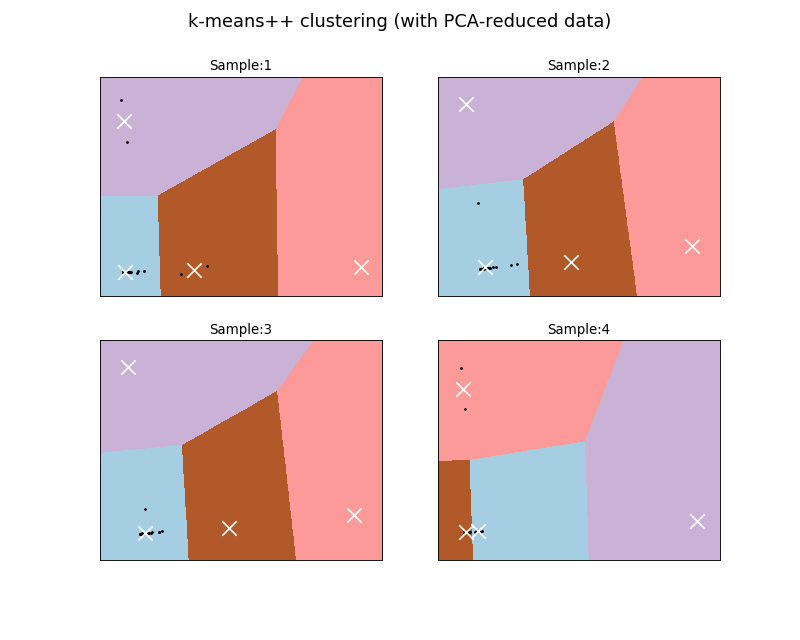
\includegraphics[width=0.90\textwidth]{kemans-clustering.png}
\caption{Clustering using k-means++ algorithm} \label{fig:k-means-clustering}
\end{figure}

k-means++ algorithm gives label to each training example. This label is the cluster number to which that training example has been assigned to. So the new labeled data look like below (table \ref{table:labeled-set}).

\begin{table}[H]
\centering
  \begin{tabular}{| l | c | c | c | c |}
    \hline
    {Destination IP Address}  &ICMP  &TCP &UDP  &Cluster \\
    \hline
    172.217.10.134  & 0     & 8     & 12  &1  \\ \hline
    65.19.96.252    & 5     & 0     & 192 &0  \\ \hline
    68.67.178.134   & 0     & 78    & 0   &2  \\ \hline
  \end{tabular}
\caption{Labeled Training Set (with cluster number)} \label{table:labeled-set}
\end{table}

We also checked the clustering accuracy using the Rand Index explained in the section \ref{subsec:Clustering} on page \pageref{subsec:Clustering}. We observed that, with more training sets, the RI index improves. A tag file which contains IP addresses, their cluster labels and average packet count is created. This tag file will be used for detecting anomaly in the network traffic.

As explained in the the section \ref{subsec:Anomaly_Detection} on page \pageref{subsec:Anomaly_Detection}, we used the training sets, that are labeled with cluster number, to get classifiers. We are using Scikit-learn's `OneClassSVM' library to train the model and create classifier for each cluster. The input vector to the classifier is the set of all the training examples belonging to the same cluster. Thus, for our four clusters, we have four classifier. The input vector to the classifier will be of the form shown in table \ref{table:labeled-set} on page \pageref{table:labeled-set}.

Following is the result of modeling on the training data sets. Each cluster has it own model. We used PCA component analysis to draw the model.

\begin{figure}[H]
\centering
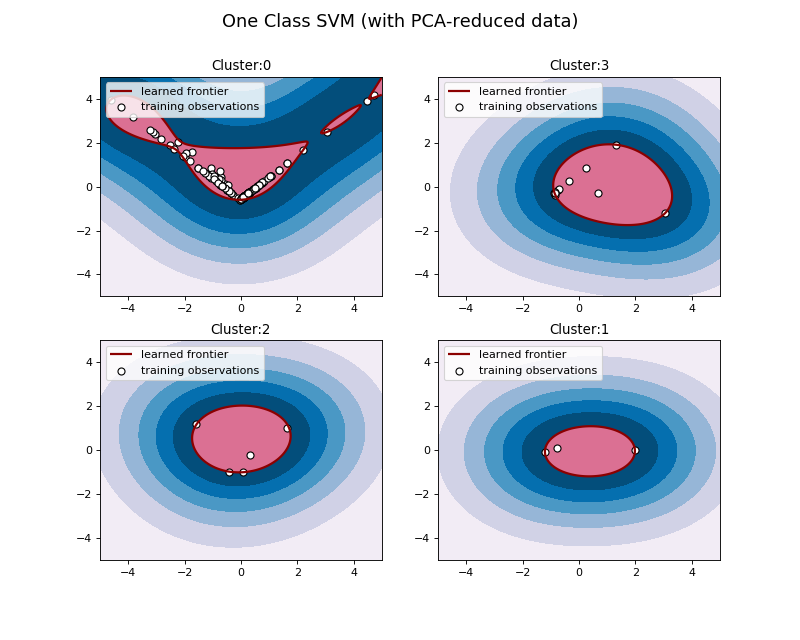
\includegraphics[width=0.80\textwidth]{one-class-SVM.png}
\caption{One Class SVM} \label{fig:one-class-SVM}
\end{figure}

At the end of the training, we have a file containing the IP addresses labeled with the cluster numbers and four classifiers for four clusters.

We took the test set which was created by capturing packets during the orchestrated DDoS attack, and used detection techniques explained in section \ref{sec:Detection} on page \pageref{sec:Detection}. Using the detection techniques on our data, we have successfully detected an attack on the destination IP address 92.168.0.7 in our modeled network.

\begin{figure}[H]
\centering
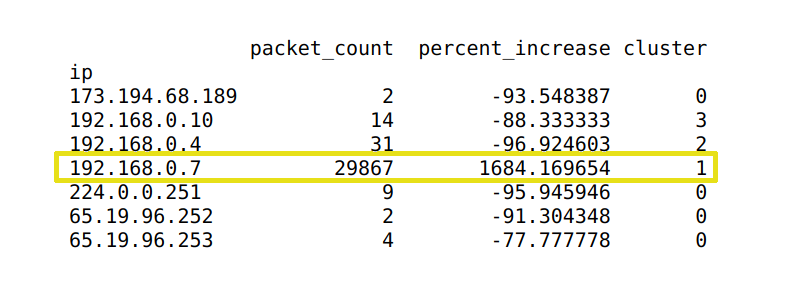
\includegraphics[width=0.80\textwidth]{detected_IP.png}
\caption{Program output} \label{fig:detected_IP}
\end{figure}

\section{Mitigation}

By now we have a computer program (consist of few modules, e.g. clustering, classification, detection) which can be run on a router and can be used to detect a DDoS attack. As there are many routers through which a destination can be reached, so to correctly detect DDoS attack we should have this programs on every router in the Internet. One of the way to achieve this is by using Network Function Virtualization (NFV)\cite{nfv}. NFV is an advanced technology which allows us to manage network devices remotely and also allows to add functionality to those networking devices. Because of this virtual technology, we don't have to manually install computer programs on the routers rather we can do it any time from anywhere. Although this technology is new, its spreading very fast and soon will be available for every commercial router.

After detecting an attack, a router can choose to block all the packets going to the destination under attack, or it can communicate the attack information to the destination. A destination can be a server or a router. The attack information can contain region name and packet count. Region is the geographical location where the router is situated and packet count is the average number of packets observed at the router for the destination during attack. Communicating the attack information to the destination can be more helpful, because the destination will be aware of the nature of the attack, i.e. for the information provided by router it will know from where attack is originated and how intense the attack is. The destination can also query router for more information such as IP source of the attack packets.

The control of blocking traffic at router can also be given to the destination. In this case, destination can perform its own analysis, understand the nature of the attack and then decide whether to block or not the incoming packets on the router. There can be different parameter based on which the destination server can decide blocking the flow and those can be provided by the router as additional information. Many questions, such as, how many routers have reported the change in traffic?, Is the attack information coming from the region which never had traffic in the past? can be asked before making the decision at the destination.

\begin{figure}[H]
\centering
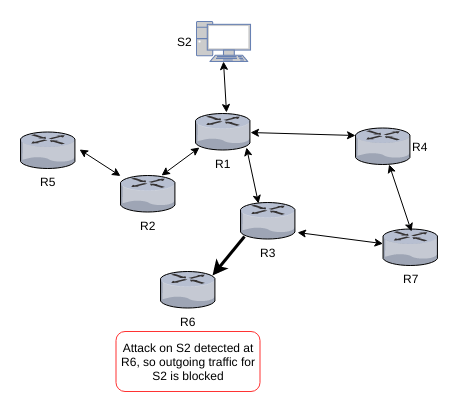
\includegraphics[scale=0.60]{mitigation_path}
\caption{Blocking traffic at router: The out-bound traffic for S2 is blocked from router R6,
because attack has been detected. While traffic from all other routers is unaffected} \label{fig:mitigation_path}
\end{figure}

To Communicate the destination network about the attack, router can use the existing ICMP protocol. ICMP protocol is used to provide feedback about the problems in the communication environment. ICMP messages are sent in several situations such as: 1) when a datagram cannot reach its destination. 2) when the gateway does not have the buffering capacity to forward a datagram. 3) when the gateway can direct the host to send traffic on a shorter route.\cite{icmp} Similarly we can use ICMP protocol to inform destination about anomalies in the traffic. ICMP protocol has many unused type code (there can be 0-255 types but as of now only 0-41 are in use). We can create a new ICMP `type' to send DDoS detection information from the router to the destination server and then destination server can send mitigation instructions to the routers.

\begin{figure}[H]
\centering
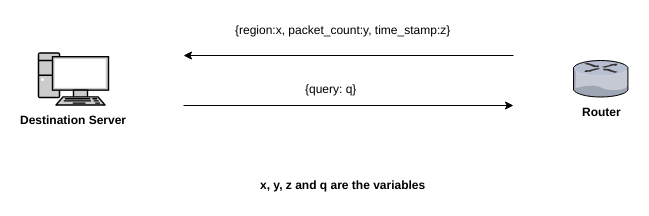
\includegraphics[scale=0.5]{router-network-communication}
\caption{Communication between a router and a destination server} \label{fig:router-network-communication}
\end{figure}

\section{Conclusion}
We have found that the DDoS attack is a real threat to every one on the Internet, and its detection is difficult because of the spoofing techniques employed by attackers. We discussed how we can combine two machine learning methods (clustering and classification) to efficiently detect DDoS attacks at the router. We also discussed that, the program which uses these algorithms can be installed on the router, thus eliminate the need for extra infrastructure for detection of a DDoS attack. With the advancement of Network Function Virtualization (NFV), it is easy to push the learning programs on the routers. We have also discussed how a router can stop an attack and also how it can communicate the attack information with the stake holders (e.g. server) for better decisions on blocking the attack traffic.

\pagebreak

\singlespacing
\bibliographystyle{unsrt}   % Unsorted order
\bibliography{biblo}       % expects file "biblo.bib"

\end{document}
